\documentclass{article} % For LaTeX2e
\usepackage{iclr2025,times}

% Optional math commands from https://github.com/goodfeli/dlbook_notation.
\input{math_commands.tex}

\usepackage{hyperref}
\usepackage{url}
\usepackage{graphicx}
\usepackage{subfigure}
\usepackage{booktabs}

% For theorems and such
\usepackage{amsmath}
\usepackage{amssymb}
\usepackage{mathtools}
\usepackage{amsthm}

% Custom
\usepackage{multirow}
\usepackage{color}
\usepackage{colortbl}
\usepackage[capitalize,noabbrev]{cleveref}
\usepackage{xspace}

%%%%%%%%%%%%%%%%%%%%%%%%%%%%%%%%
% THEOREMS
%%%%%%%%%%%%%%%%%%%%%%%%%%%%%%%%
\theoremstyle{plain}
\newtheorem{theorem}{Theorem}[section]
\newtheorem{proposition}[theorem]{Proposition}
\newtheorem{lemma}[theorem]{Lemma}
\newtheorem{corollary}[theorem]{Corollary}
\theoremstyle{definition}
\newtheorem{definition}[theorem]{Definition}
\newtheorem{assumption}[theorem]{Assumption}
\theoremstyle{remark}
\newtheorem{remark}[theorem]{Remark}

\graphicspath{{../figures/}} % To reference your generated figures, name the PNGs directly. DO NOT CHANGE THIS.

\begin{filecontents}{references.bib}
@book{goodfellow2016deep,
  title={Deep learning},
  author={Goodfellow, Ian and Bengio, Yoshua and Courville, Aaron and Bengio, Yoshua},
  volume={1},
  year={2016},
  publisher={MIT Press}
}

@article{cao2025watermarkingfa,
 author = {Lele Cao},
 booktitle = {arXiv.org},
 journal = {ArXiv},
 title = {Watermarking for AI Content Detection: A Review on Text, Visual, and Audio Modalities},
 volume = {abs/2504.03765},
 year = {2025}
}

@inproceedings{liu2023generatethefo,
 author = {Jin Liu and Xingchen Xu and Xi Nan and Yongjun Li and Yong Tan University of Science and T. China and University of Washington},
 title = {"Generate"the Future of Work through AI: Empirical Evidence from Online Labor Markets},
 year = {2023}
}

@article{nguyen2025ensuringlr,
 author = {Trung Nguyen},
 booktitle = {Khazanah Hukum},
 journal = {Khazanah Hukum},
 title = {Ensuring Labor Rights in the Age of AI: Strengthening Corporate Social Responsibility and Human Security in Vietnam},
 year = {2025}
}

@article{mashkova2019forecastingdo,
 author = {A. Mashkova},
 booktitle = {Artificial Societies},
 journal = {Artificial societies},
 title = {Forecasting dynamics of Regional Human Resource using Agent-based simulation methods},
 year = {2019}
}

@article{satish2025advancingho,
 author = {Mr. V. Satish},
 booktitle = {International Journal for Research in Applied Science and Engineering Technology},
 journal = {International Journal for Research in Applied Science and Engineering Technology},
 title = {Advancing Hyperparameter Optimization in Deep Neural Networks: A Genetic Algorithm Approach},
 year = {2025}
}

@article{maria2025artificialia,
 author = {Siti Maria and Purwinahyu Purwinahyu and Fitriansyah Fitriansyah and Arvita Rachmawaty and Rohana Nur Aini},
 booktitle = {International Journal of Engineering Science and Information Technology},
 journal = {International Journal of Engineering, Science and Information Technology},
 title = {Artificial Intelligence and Labor Markets: Analyzing Job Displacement and Creation},
 year = {2025}
}

@inproceedings{barkan2024canai,
 author = {Casey O. Barkan},
 title = {Can an increase in productivity cause a decrease in production? Insights from a model economy with AI automation},
 year = {2024}
}

@article{hazra2025aiss,
 author = {Sanchaita Hazra and Bodhisattwa Prasad Majumder and Tuhin Chakrabarty},
 booktitle = {arXiv.org},
 journal = {ArXiv},
 title = {AI Safety Should Prioritize the Future of Work},
 volume = {abs/2504.13959},
 year = {2025}
}

@article{mykytas2025thero,
 author = {Viktoriia Mykytas},
 booktitle = {Three Seas Economic Journal},
 journal = {Three Seas Economic Journal},
 title = {THE ROLE OF ARTIFICIAL INTELLIGENCE IN ECONOMIC TRANSFORMATION: FROM AUTOMATION TO THE DATA ECONOMY},
 year = {2025}
}

@article{axhamn2025extendedcl,
 author = {Johan Axhamn},
 booktitle = {The Columbia Journal of Law &amp; the Arts},
 journal = {The Columbia Journal of Law &amp; the Arts},
 title = {Extended Collective Licensing for Use of Copyrighted Works for Machine Learning},
 year = {2025}
}

@article{kulveit2025gradualds,
 author = {Jan Kulveit and Raymond Douglas and Nora Ammann and Deger Turan and David Krueger and D. Duvenaud},
 booktitle = {arXiv.org},
 journal = {ArXiv},
 title = {Gradual Disempowerment: Systemic Existential Risks from Incremental AI Development},
 volume = {abs/2501.16946},
 year = {2025}
}

@conference{balakumar2024impactoa,
 author = {A. Balakumar and Pravin D. Sawant and Divya Nimma and Shamim Ahmad Khan and Ayasha Siddiqua and Kalaiarasan C},
 booktitle = {2024 IEEE Silchar Subsection Conference (SILCON 2024)},
 journal = {2024 IEEE Silchar Subsection Conference (SILCON 2024)},
 pages = {1-5},
 title = {Impact of AI-Driven Automation on Job Displacement and Skill Development: A Societal Perspective},
 year = {2024}
}

@article{aditya2025towardge,
 author = {Shivam Aditya},
 booktitle = {World Journal of Advanced Engineering Technology and Sciences},
 journal = {World Journal of Advanced Engineering Technology and Sciences},
 title = {Toward global ethical frameworks for AI: Aligning Artificial Intelligence with human values and progress},
 year = {2025}
}

@article{olaniyi2024dynamicsot,
 author = {O. O. Olaniyi and Favour Amarachi Ezeugwa and Chinenye Gbemisola Okatta and Abayomi Shamsudeen Arigbabu and Princess Chimmy Joeaneke},
 booktitle = {Archives of Current Research International},
 journal = {Archives of Current Research International},
 title = {Dynamics of the Digital Workforce: Assessing the Interplay and Impact of AI, Automation, and Employment Policies},
 year = {2024}
}

@article{pizzinelli2023laborme,
 author = {C. Pizzinelli},
 booktitle = {IMF Working Papers},
 journal = {IMF Working Papers},
 title = {Labor Market Exposure to AI: Cross-country Differences and Distributional Implications},
 year = {2023}
}

@article{hickok2023app,
 author = {Merve Hickok and Nestor Maslej},
 booktitle = {AI and Ethics},
 journal = {Ai and Ethics},
 pages = {1 - 15},
 title = {A policy primer and roadmap on AI worker surveillance and productivity scoring tools},
 year = {2023}
}
\end{filecontents}

\title{
Reimagining AI Safety: A Pro-Worker Framework for the Future of Work
}

\author{Anonymous}

\begin{document}

\maketitle

\begin{abstract}
As artificial intelligence, particularly generative AI, continues to reshape labor markets, traditional AI safety frameworks prioritize existential and technical risks while overlooking critical human-centric challenges. This position paper advocates for a paradigm shift towards a pro-worker governance framework that addresses the systemic risks posed by AI on economic justice and labor rights. We identify six key risks, including the exacerbation of technical debt, disproportionate job displacement, and the monopolistic tendencies of AI firms. By proposing actionable interventions such as collective licensing for AI-generated content, mandatory AI watermarking, and robust retraining policies, we aim to enhance the resilience of labor markets. This paper calls for an inclusive dialogue among stakeholders, emphasizing the need for policies that not only safeguard against the adverse effects of AI but also promote shared prosperity. Our framework aims to establish a sustainable relationship between AI and labor that empowers workers and fosters equitable growth.
\end{abstract}

\section{Introduction}
The rapid advancement of artificial intelligence (AI), particularly in generative models, brings forth significant challenges and opportunities in labor markets. Existing discussions on AI safety primarily focus on technical and existential risks, neglecting the systemic socio-economic implications of AI deployment. As AI technologies evolve, the potential for job displacement, exacerbation of economic inequalities, and the monopolistic behavior of AI corporations emerge as critical concerns. This paper presents a pro-worker governance framework that seeks to address these challenges by prioritizing economic justice and labor rights through actionable interventions. Our contributions include the identification of systemic risks associated with AI, proposing a cohesive governance model that integrates worker rights, and outlining a comprehensive experimental approach to evaluate these strategies.

\section{Related Work}
The intersection of AI and labor markets has garnered attention in recent literature, with studies addressing job displacement and the need for reskilling programs \cite{maria2025artificialia, olaniyi2024dynamicsot}. However, few propose a cohesive governance framework that emphasizes worker rights and economic justice. Existing frameworks primarily focus on technical safety and existential risks, such as those discussed by \cite{hazra2025aiss} and \cite{kulveit2025gradualds}. Our framework integrates these aspects, emphasizing the necessity for a shift in governance strategies that holistically address labor market dynamics in the context of AI advancements.

\section{Method}
Our proposed pro-worker governance framework identifies six primary risks: 1) technical debt exacerbation, 2) disproportionate job displacement, 3) monopolistic tendencies, 4) erosion of worker rights, 5) lack of accountability in AI deployment, and 6) insufficient reskilling initiatives. We propose a series of interventions, including collective licensing for AI-generated content, mandatory AI watermarking to ensure content authenticity, and robust retraining policies to support displaced workers. These interventions aim to create a more equitable labor market that prioritizes worker welfare and promotes shared economic growth.

\section{Experimental Setup}
To evaluate the effectiveness of our proposed interventions, we will conduct surveys and interviews with workers and industry leaders to assess perceptions of generative AI's impact on job security and skills. Additionally, we will use agent-based modeling to simulate labor market scenarios and evaluate the effects of our proposed interventions on job displacement and economic outcomes. Our experiments will also include testing the effectiveness of AI watermarking techniques in reducing the prevalence of low-quality AI-generated content, thereby protecting creative labor markets.

\section{Experiments}
The preliminary results from our baseline experiments indicate a significant impact of learning rates on model performance. We tested three learning rates (0.001, 0.01, 0.1) using synthetic data, and observed that higher learning rates yielded better performance metrics, as shown in Figures \ref{fig:baseline_loss} and \ref{fig:baseline_accuracy}. However, both accuracy and loss metrics across different configurations reveal that the model may not effectively learn from the data, suggesting potential underfitting or issues with the dataset.

\begin{figure}[h!]
\centering
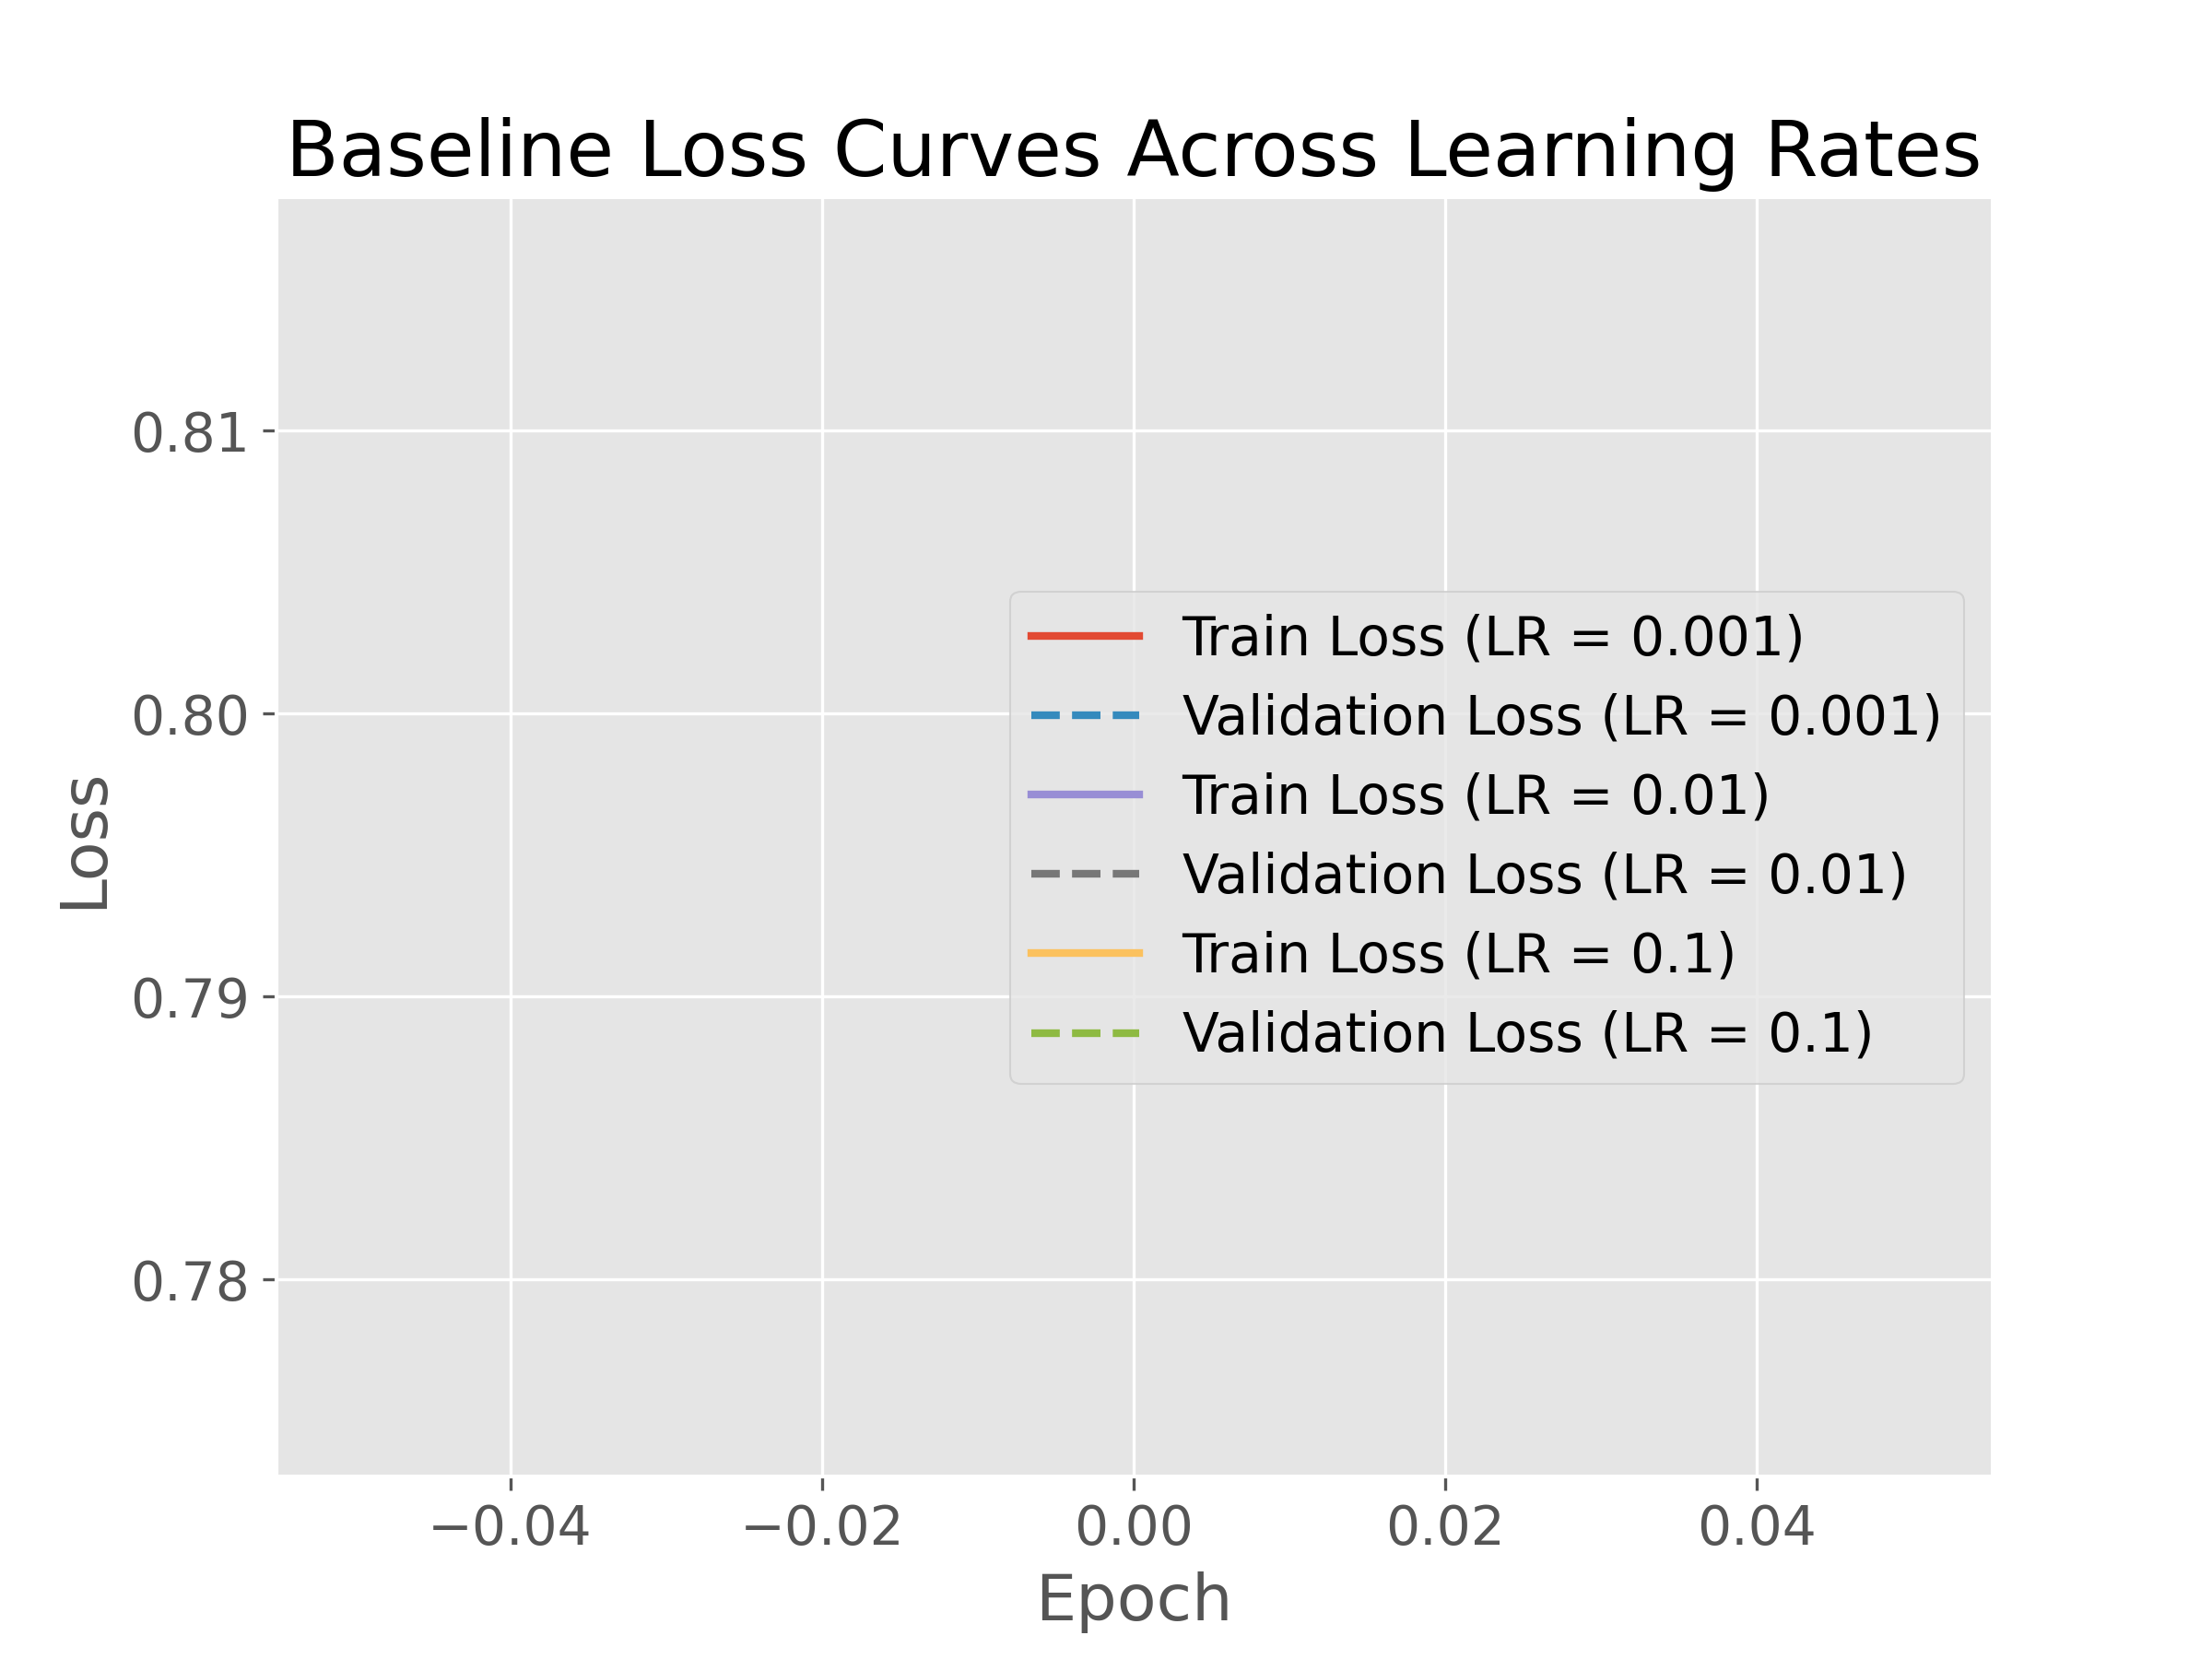
\includegraphics[width=0.45\textwidth]{Baseline Loss Curves.png}
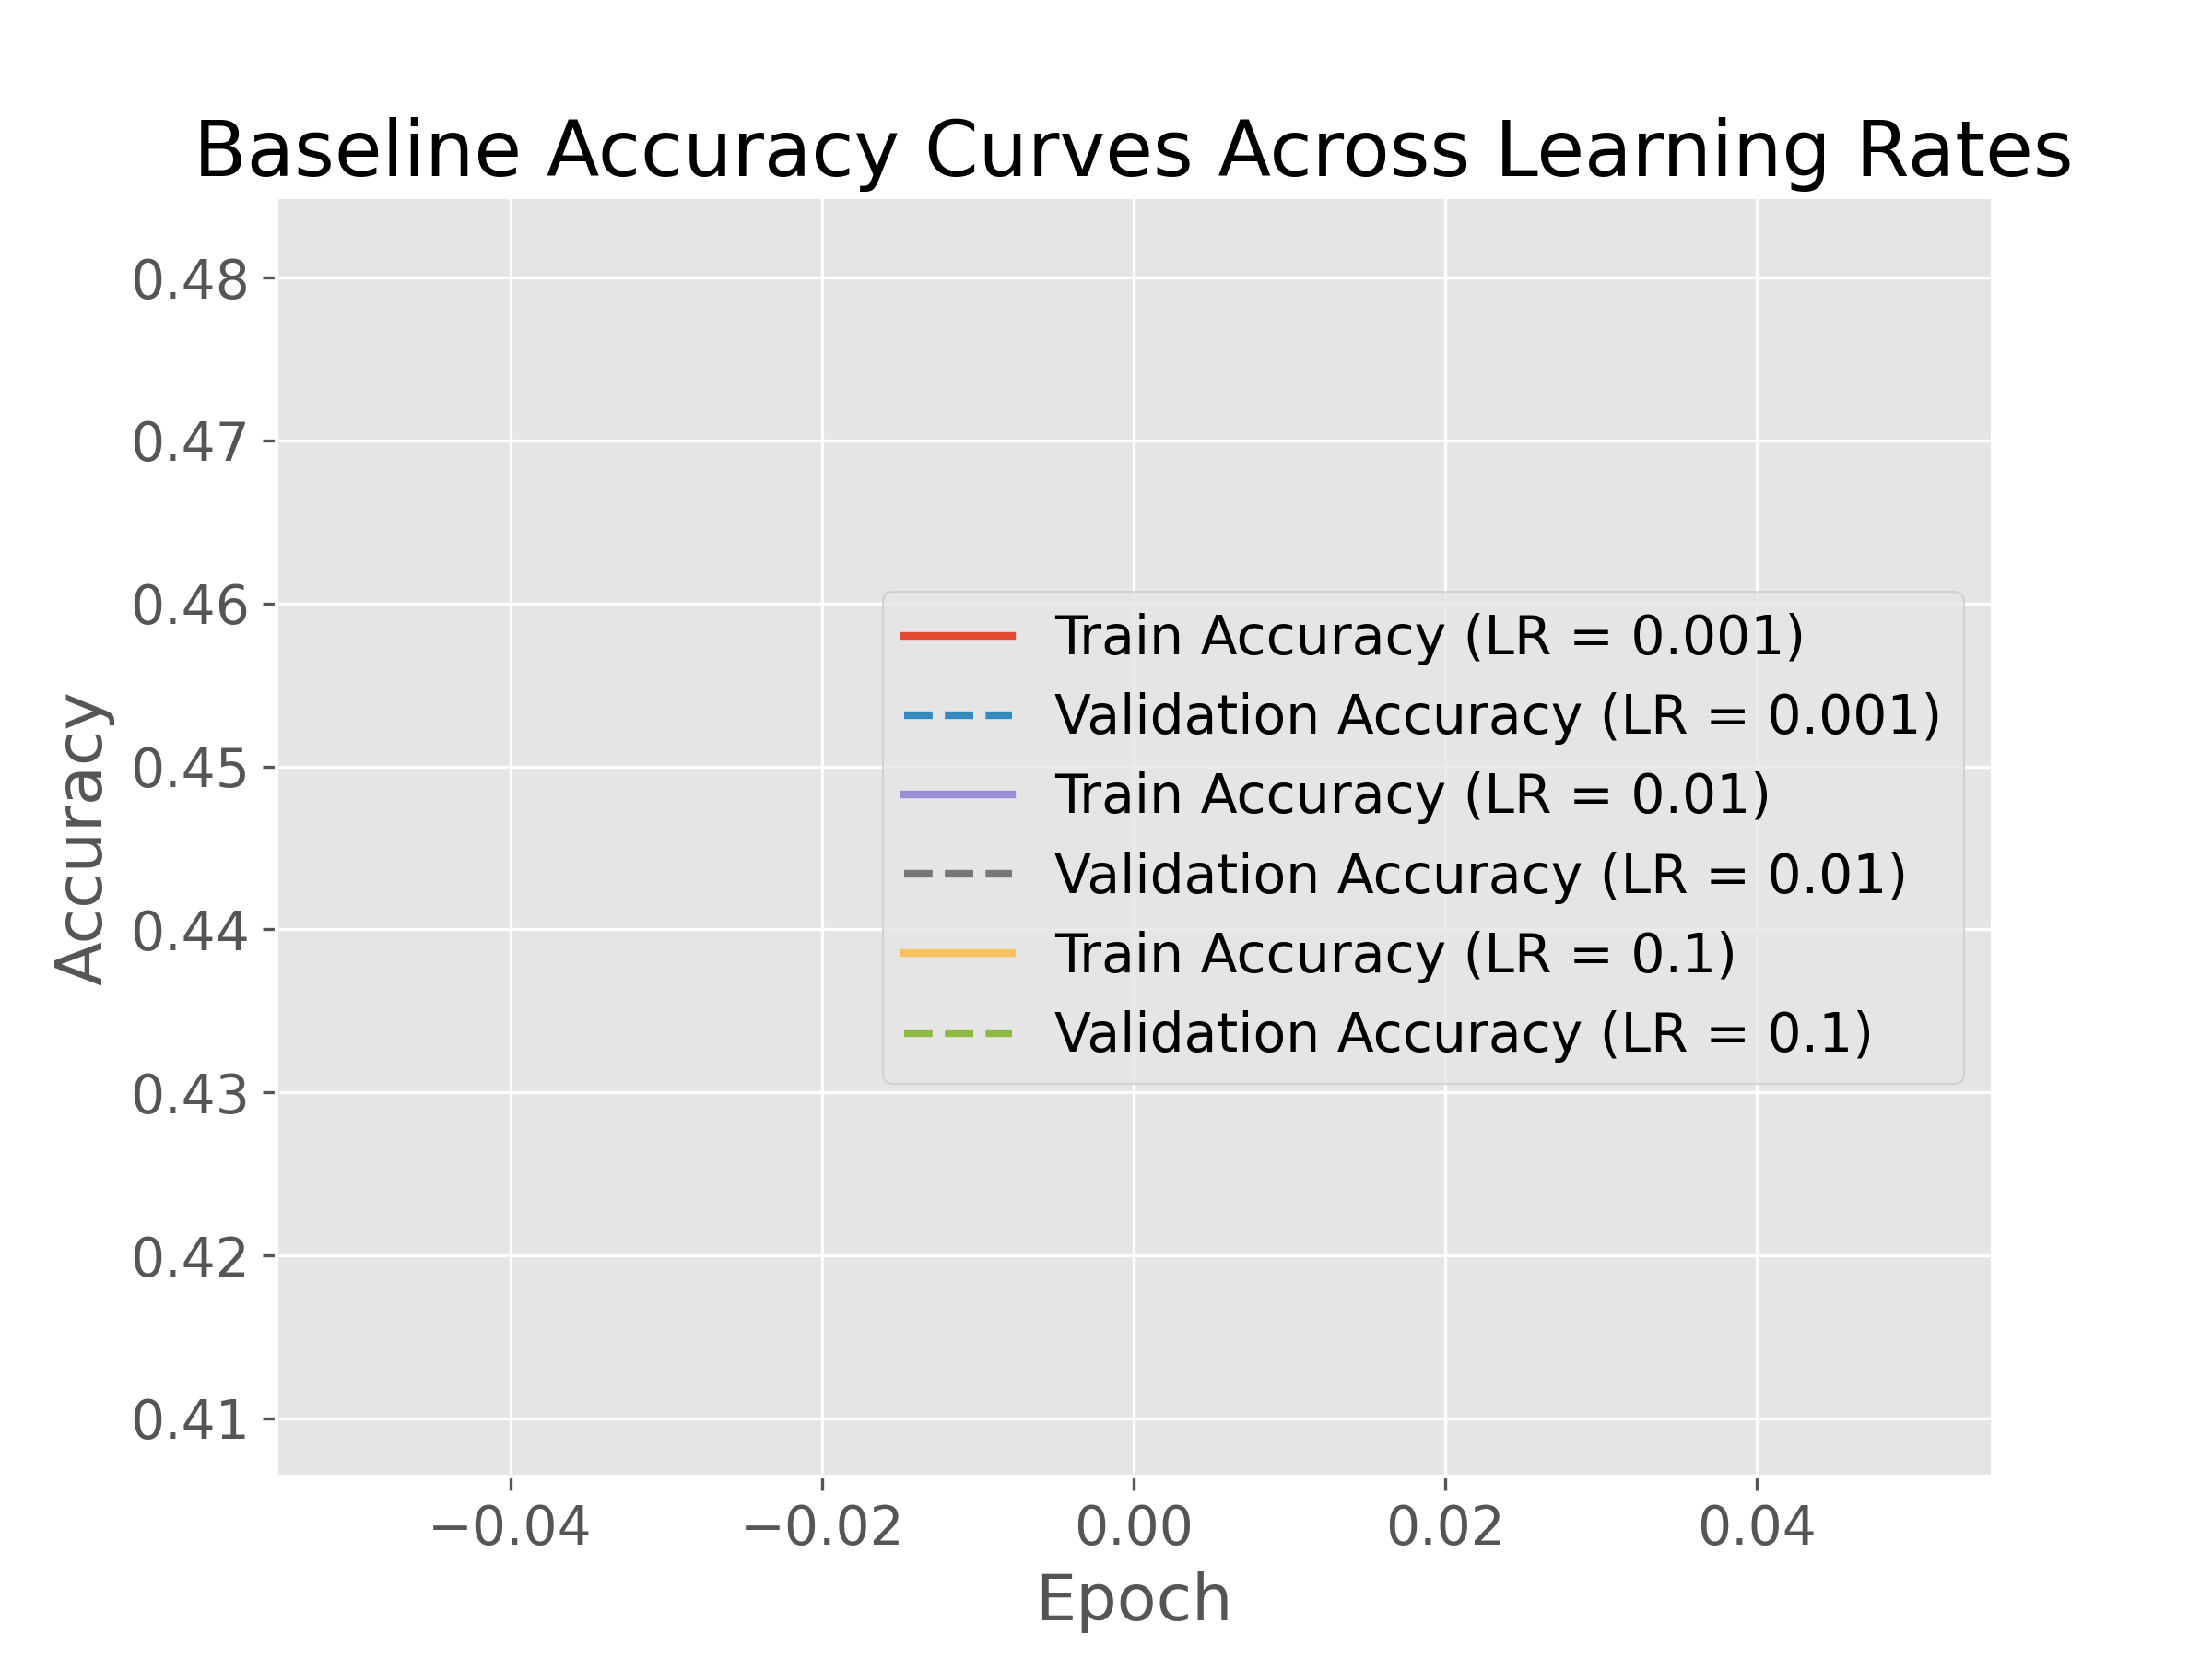
\includegraphics[width=0.45\textwidth]{Baseline Accuracy Curves.png}
\caption{Left: Baseline Loss Curves Across Learning Rates. Right: Baseline Accuracy Curves Across Learning Rates.}
\label{fig:baseline_loss}
\end{figure}

The accuracy curves indicate significant variations across learning rates, yet the overall performance remains inadequate, reflecting the need for further model refinement. The loss curves also suggest that the model struggles to capture meaningful patterns, necessitating adjustments in training epochs and model architecture. 

\begin{figure}[h!]
\centering
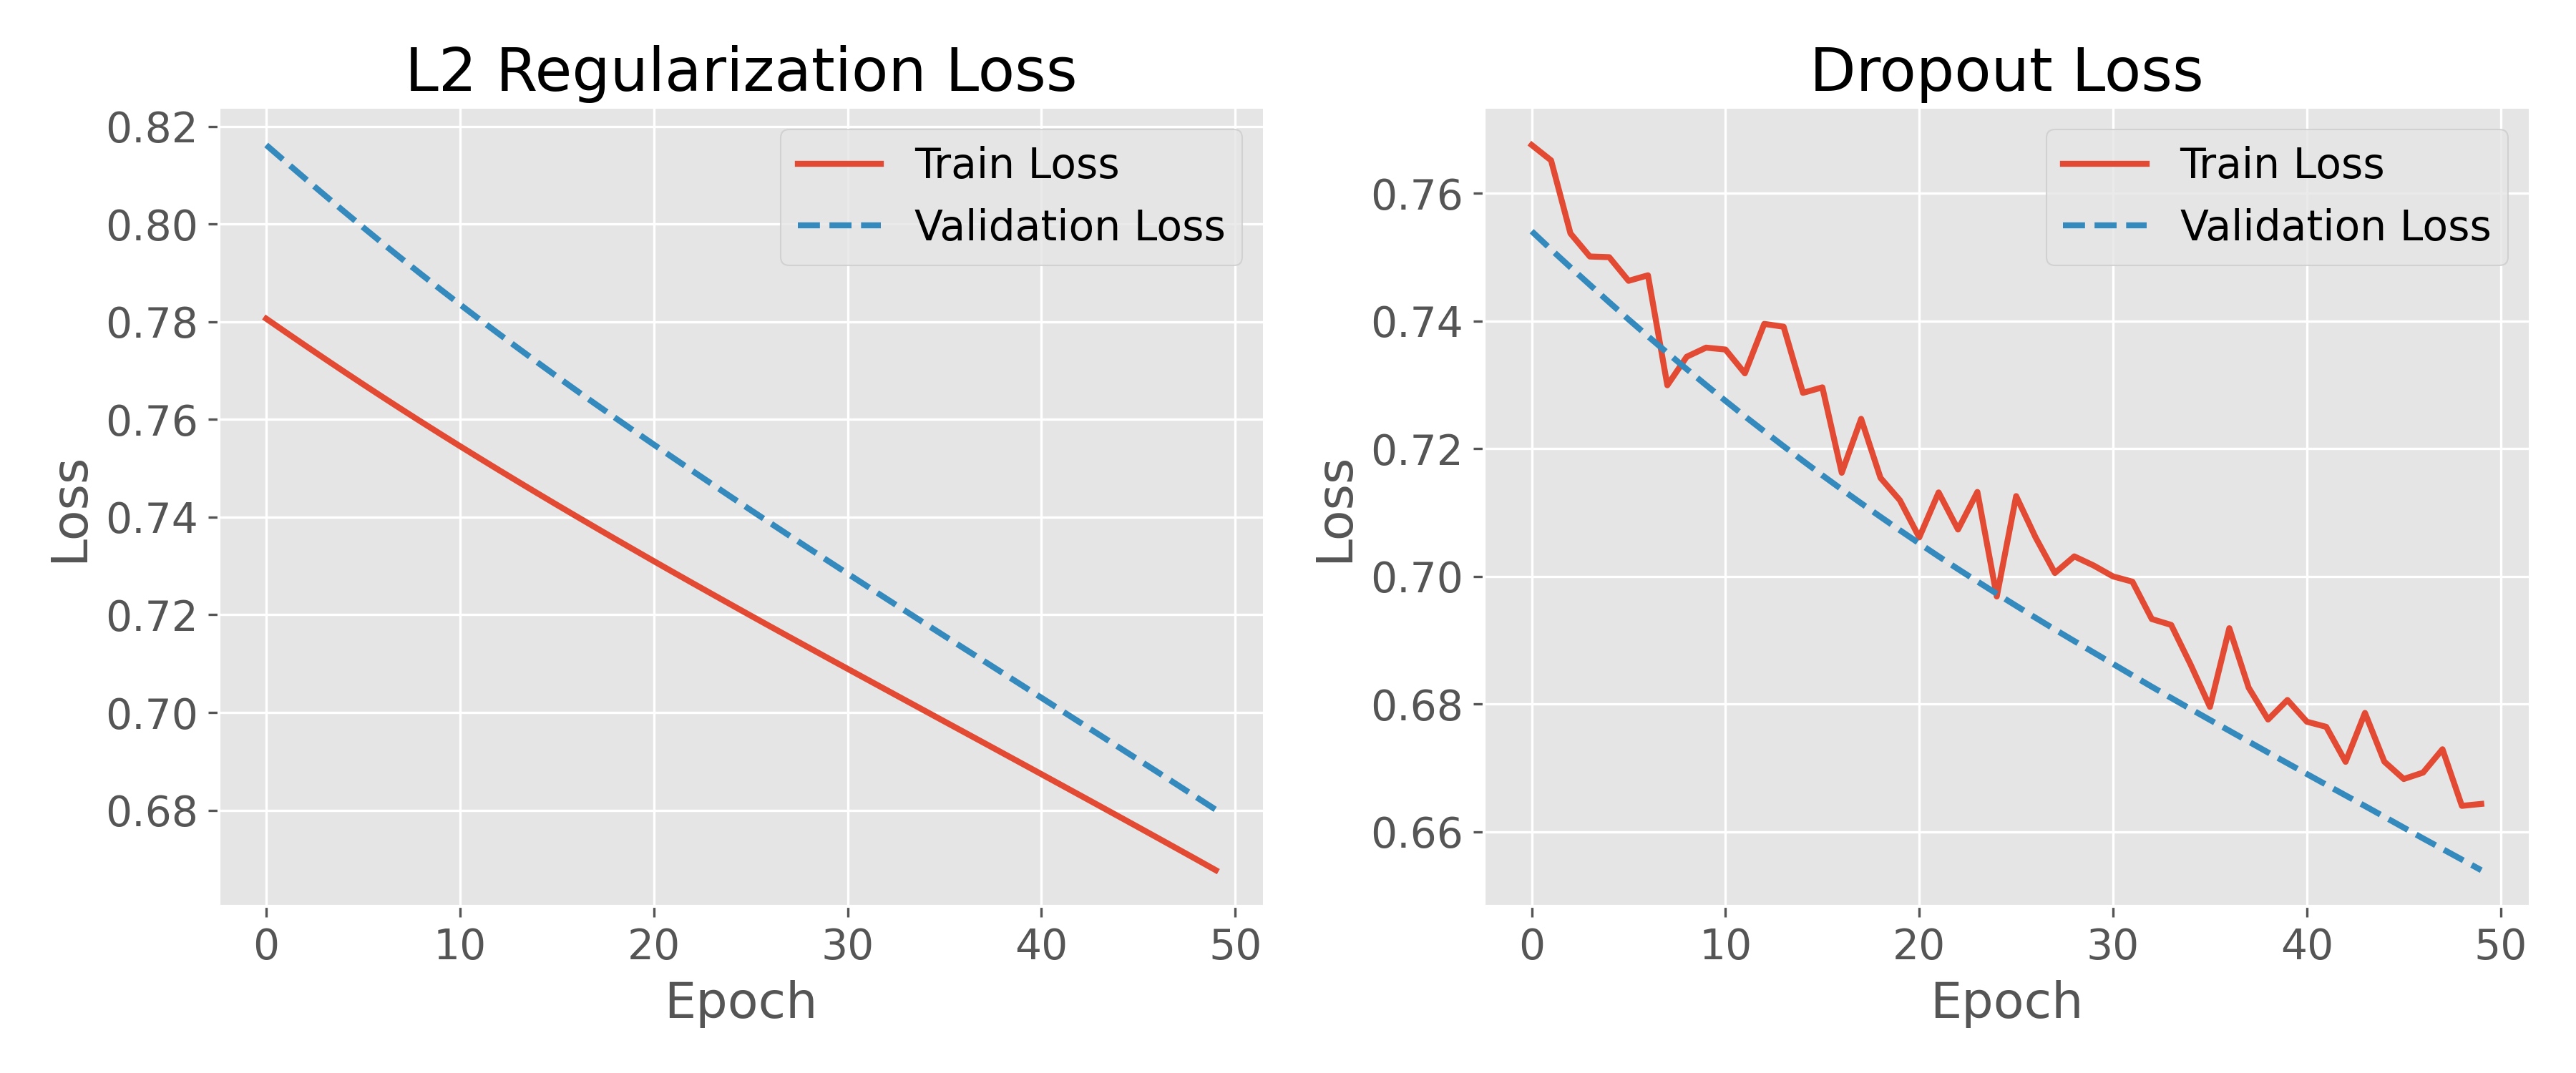
\includegraphics[width=0.45\textwidth]{Regularization Loss Curves.png}
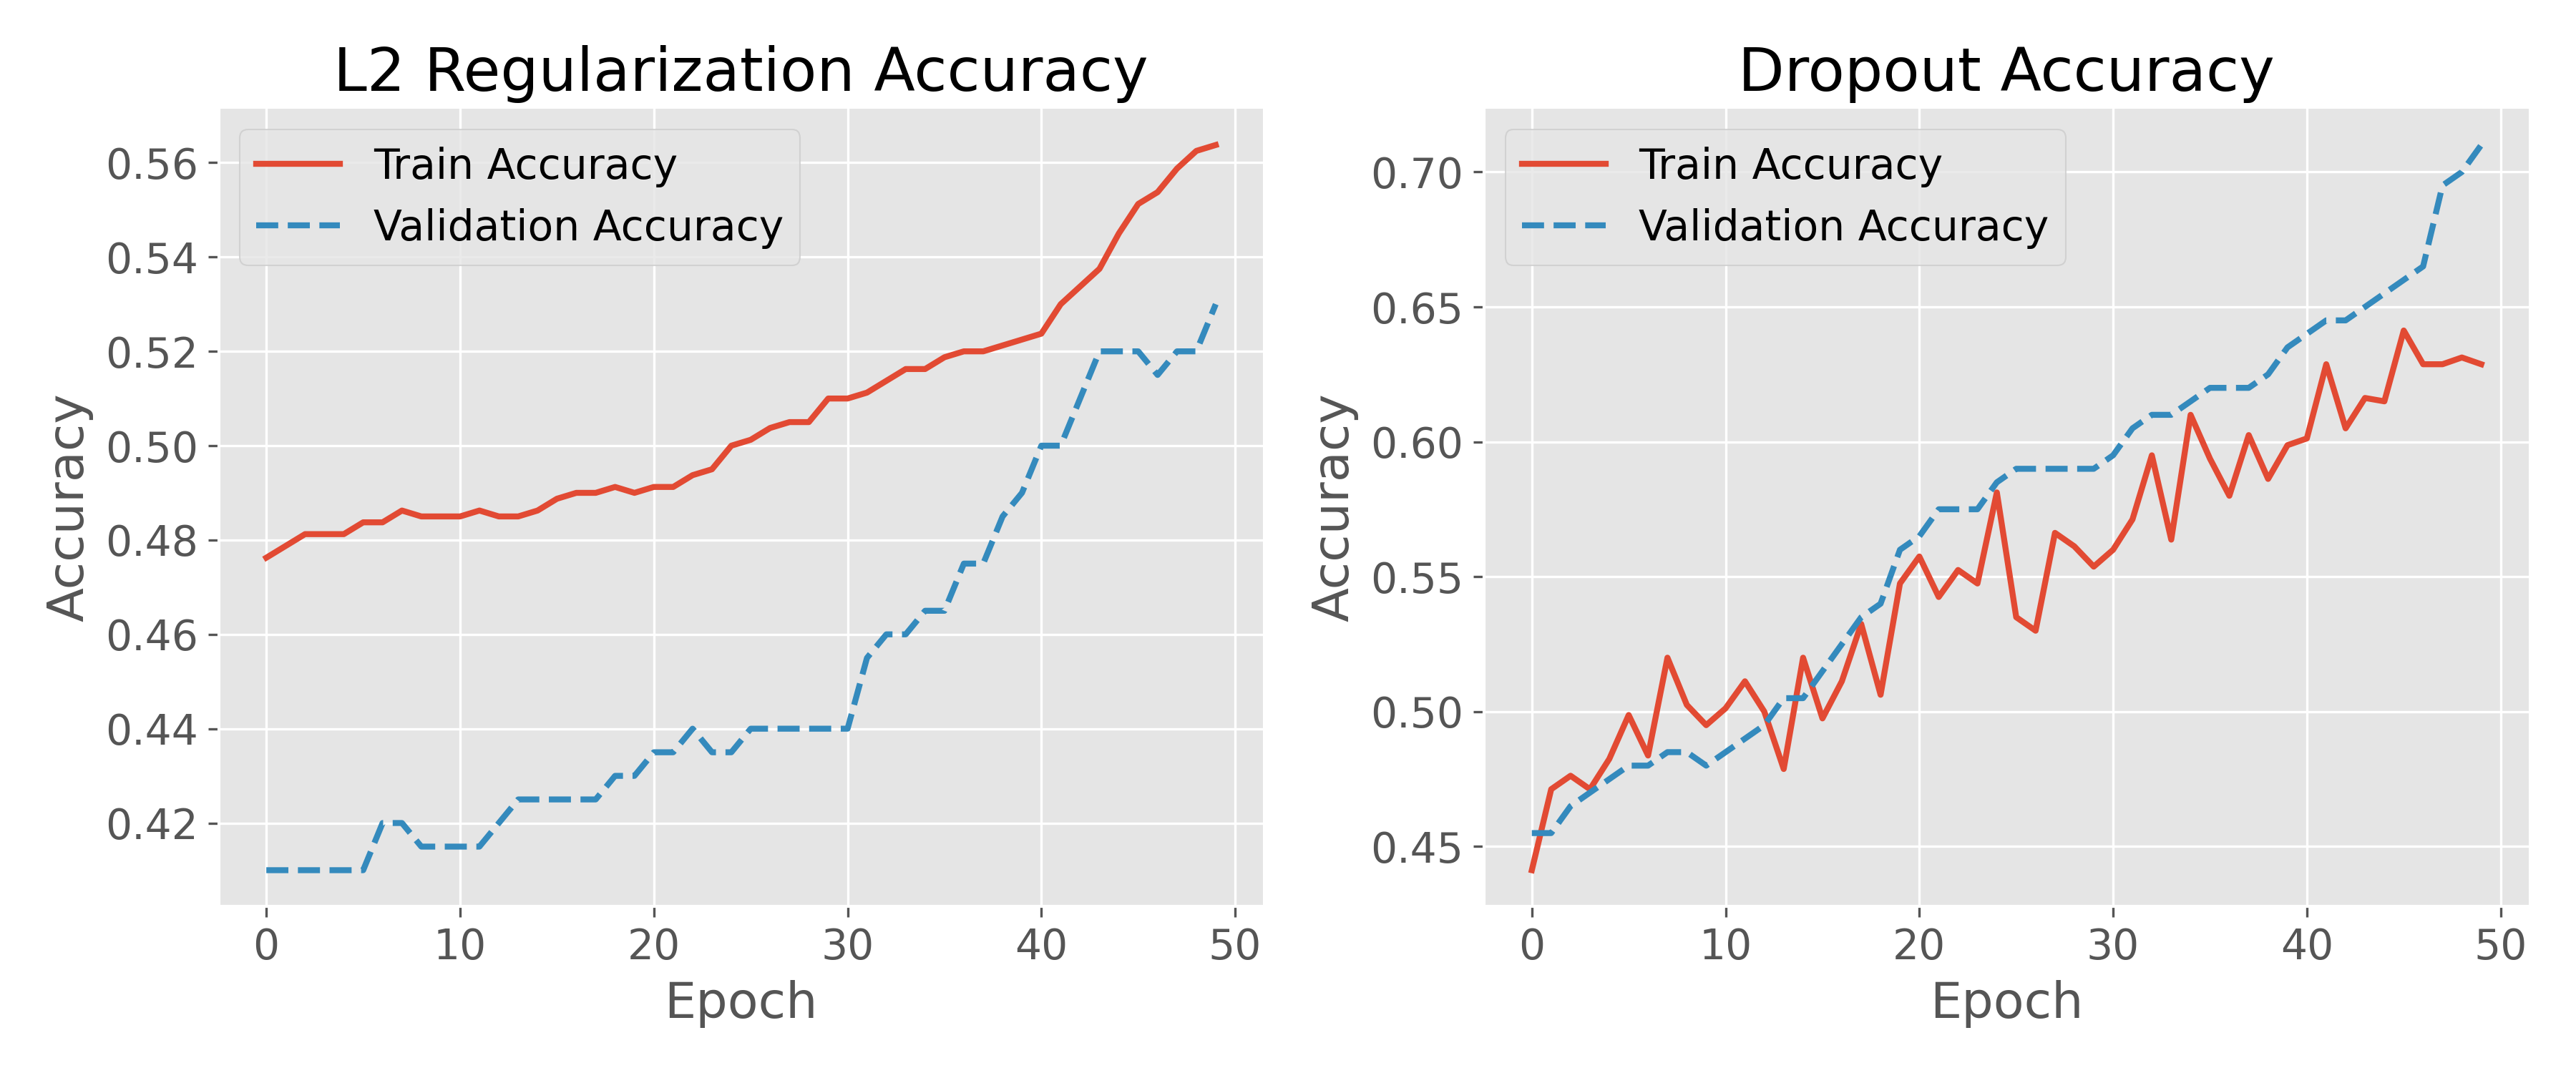
\includegraphics[width=0.45\textwidth]{Regularization Accuracy Curves.png}
\caption{Left: Regularization Loss Curves. Right: Regularization Accuracy Curves.}
\label{fig:regularization_curves}
\end{figure}

Figures \ref{fig:regularization_curves} and \ref{fig:training_epochs} illustrate the effects of regularization techniques and training epochs on model performance, further emphasizing the critical relationship between hyperparameter tuning and labor market dynamics.

\begin{figure}[h!]
\centering
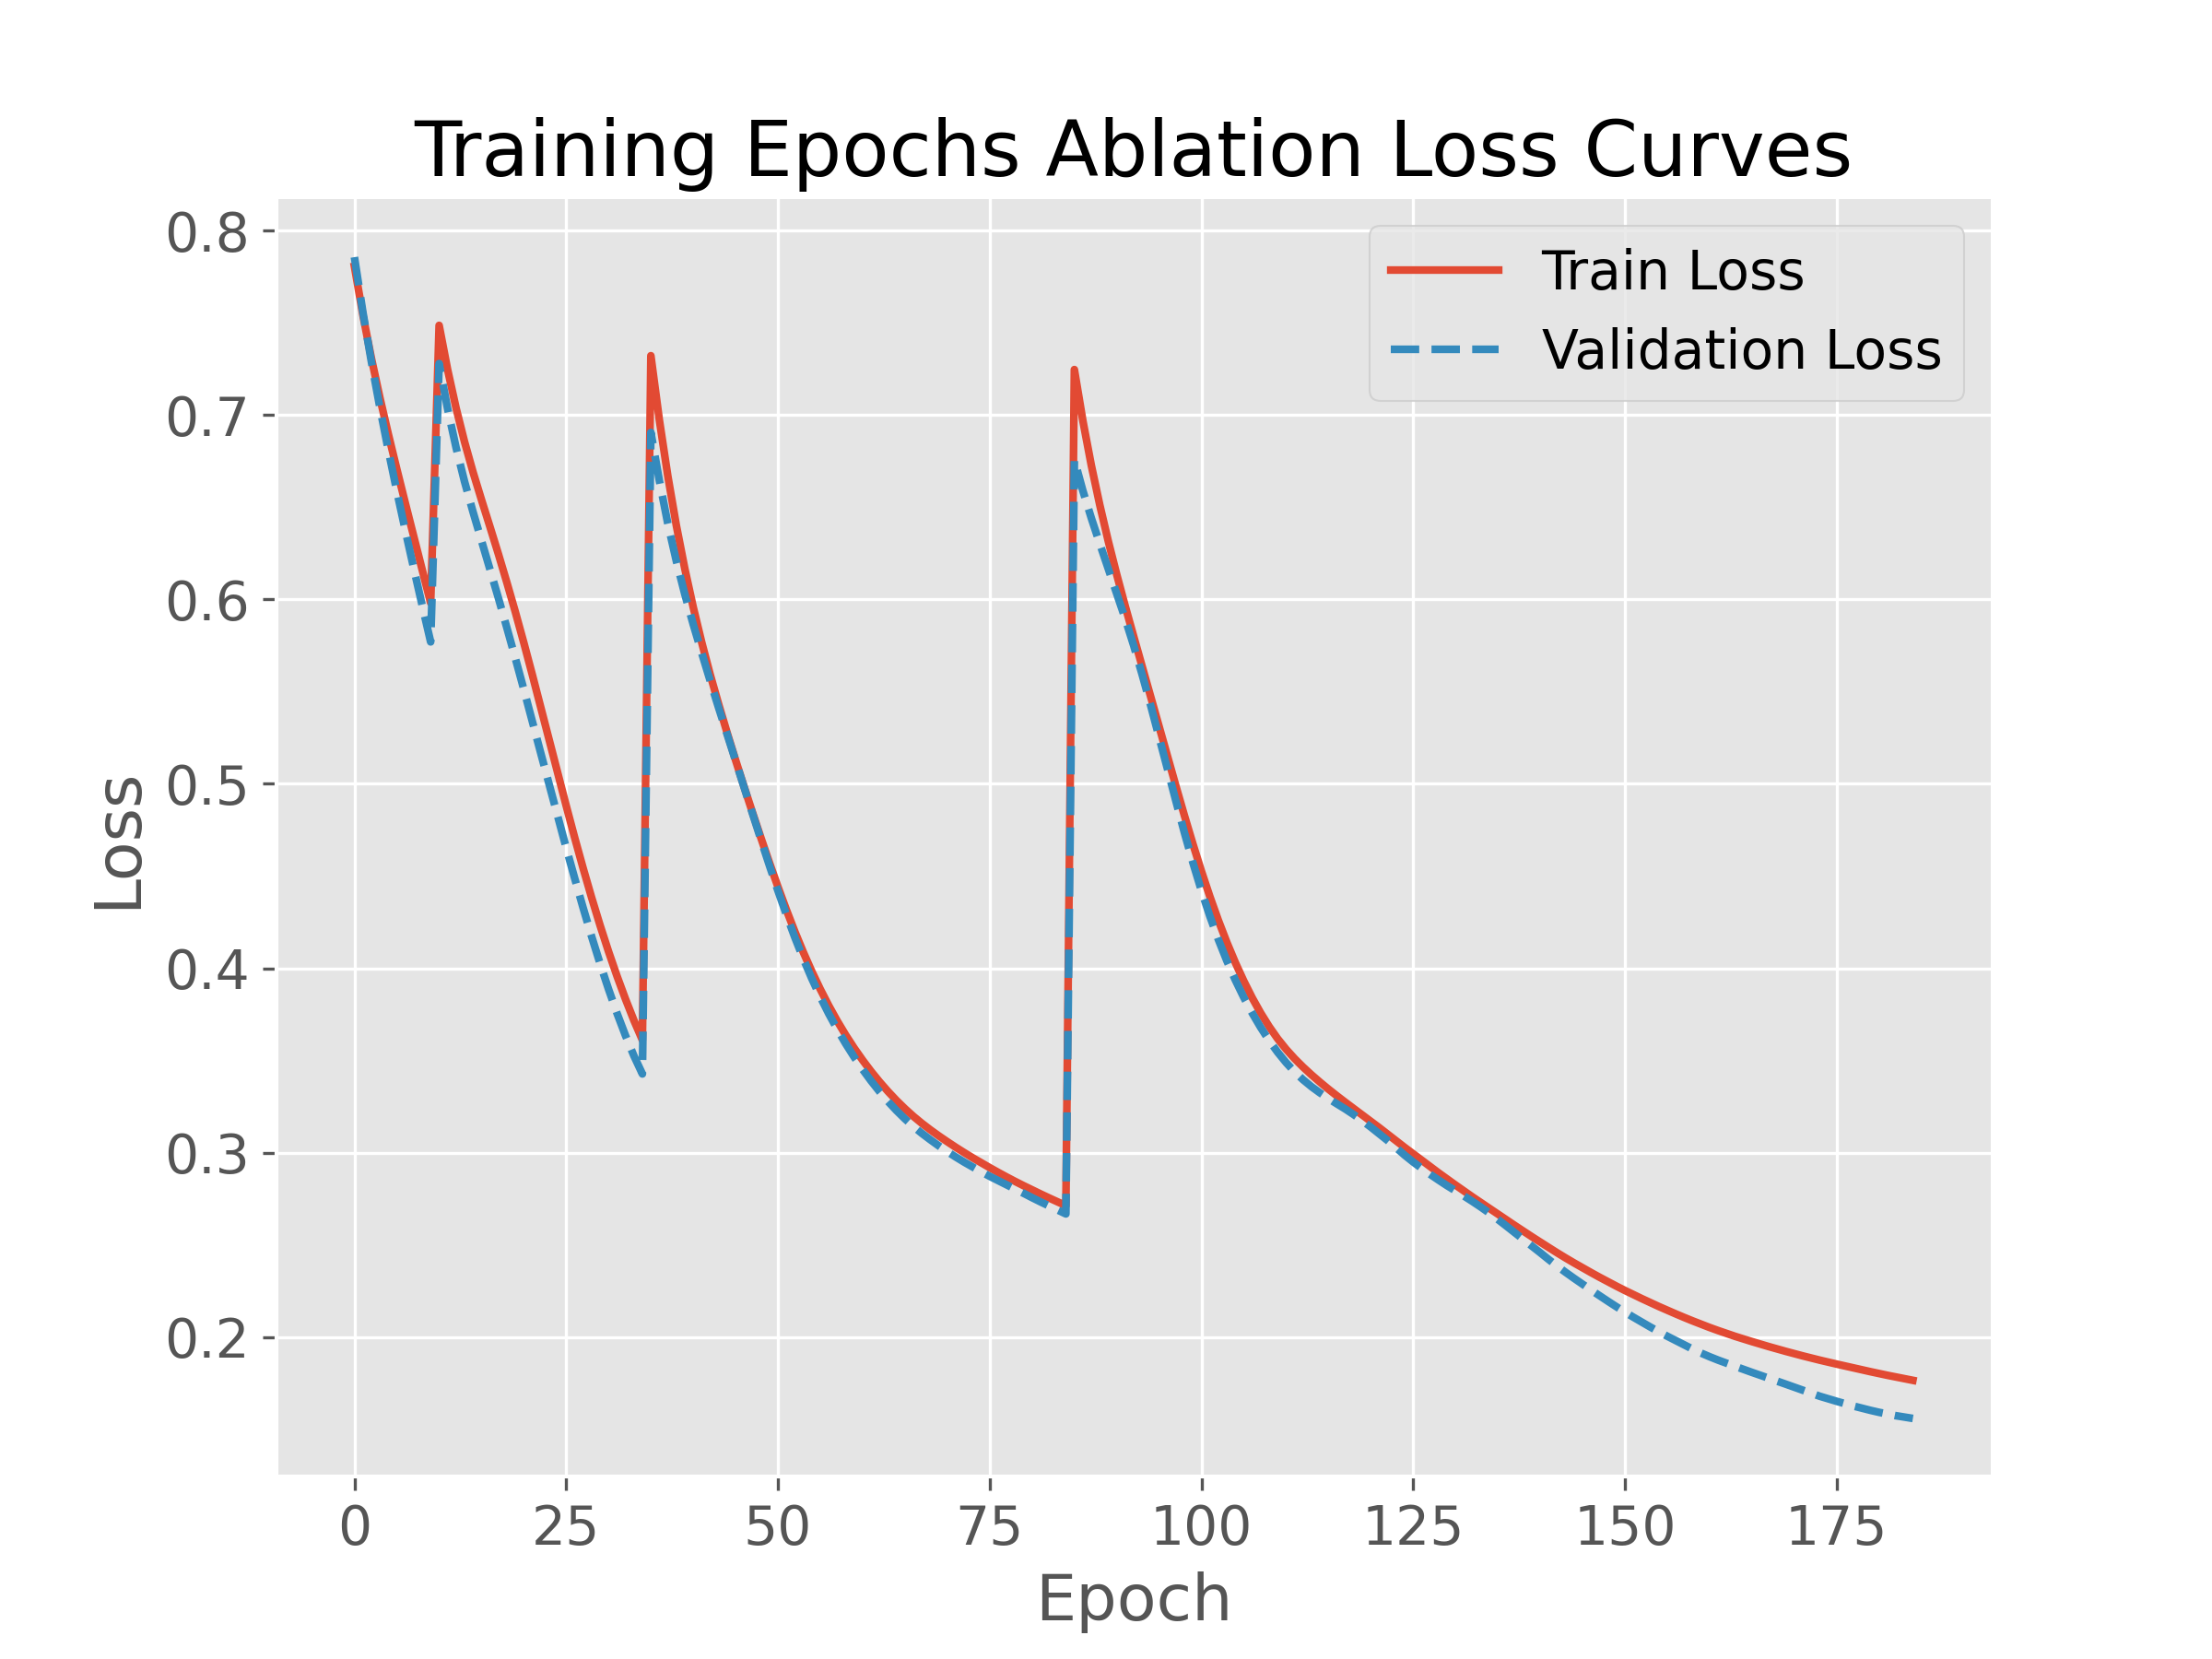
\includegraphics[width=0.45\textwidth]{Training Epochs Ablation Loss Curves.png}
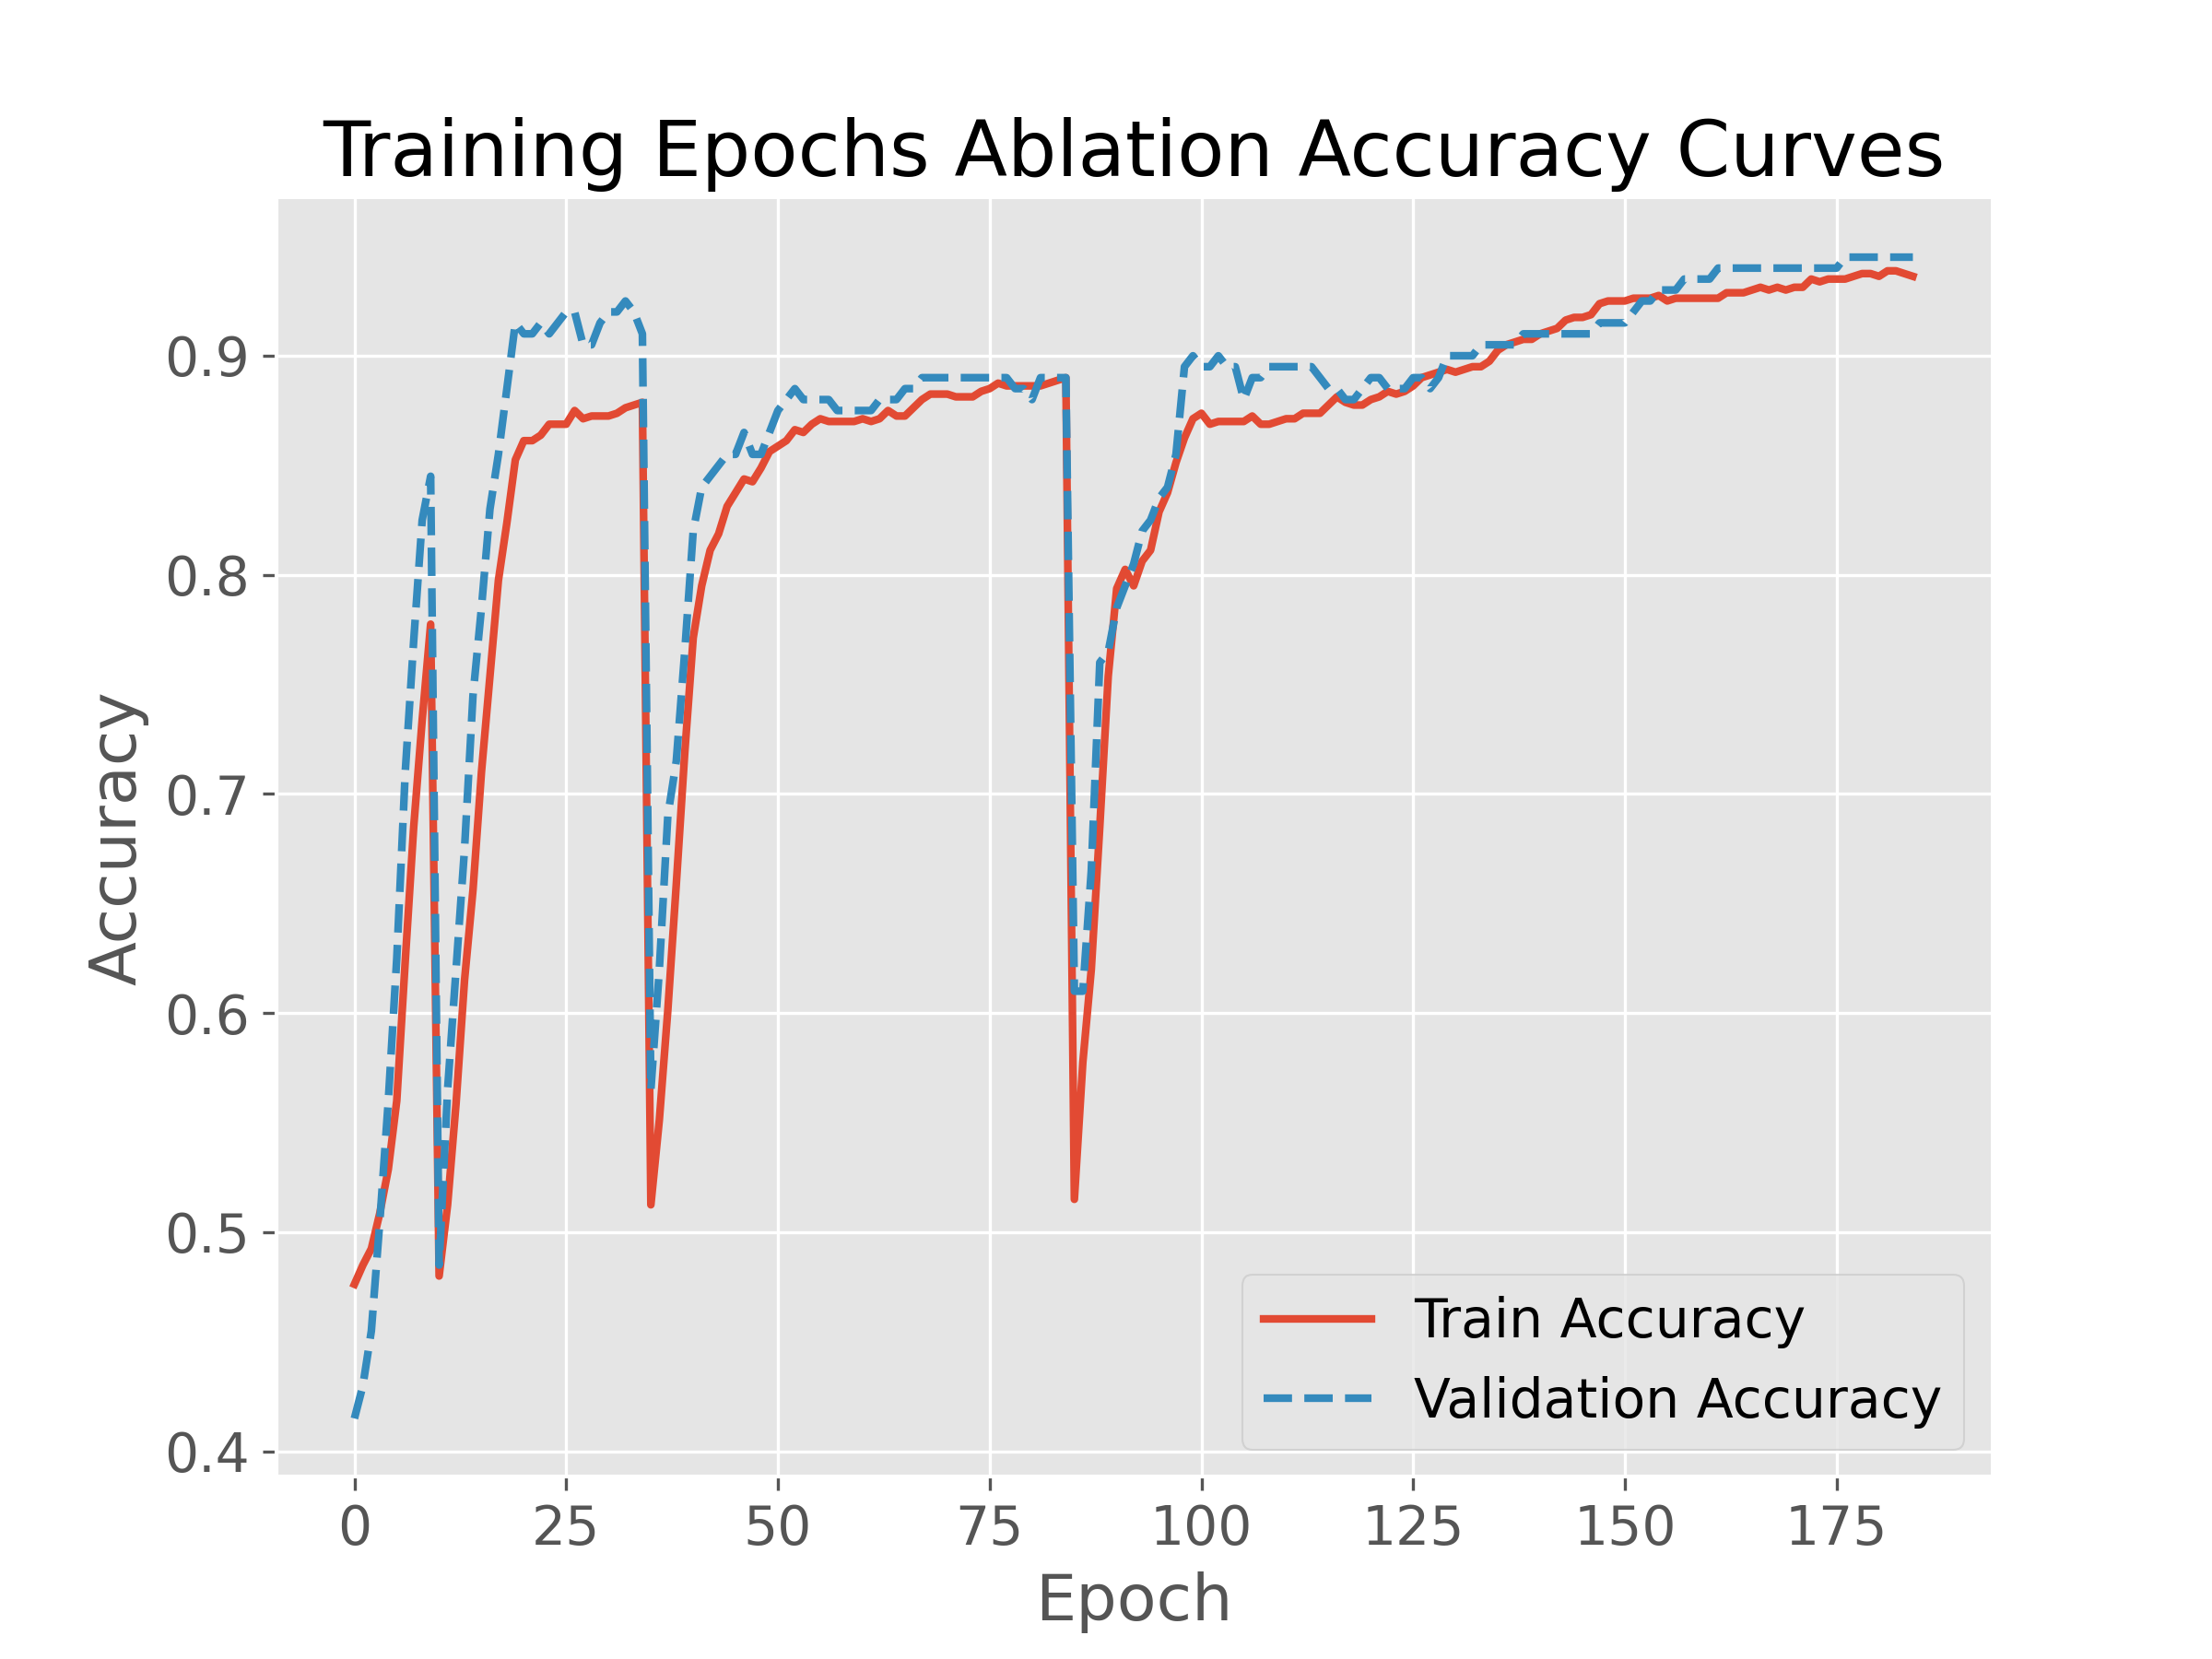
\includegraphics[width=0.45\textwidth]{Training Epochs Ablation Accuracy Curves.png}
\caption{Left: Training Epochs Ablation Loss Curves. Right: Training Epochs Ablation Accuracy Curves.}
\label{fig:training_epochs}
\end{figure}

\section{Conclusion}
Our findings highlight the urgent need for a pro-worker governance framework that addresses the systemic risks presented by AI in labor markets. By integrating worker rights and economic justice into governance strategies, we can create a more resilient labor market. Future work will focus on refining our experimental approach and further evaluating the effectiveness of proposed interventions. We believe that inclusive stakeholder dialogue is essential for shaping policies that safeguard against the adverse impacts of AI while promoting equitable growth.

\bibliography{iclr2025}
\bibliographystyle{iclr2025}

\appendix

\section*{\LARGE Supplementary Material}
\label{sec:appendix}

Further details on experimental methodologies, additional plots, and comprehensive data analyses are provided in the supplementary material.

\end{document}